\chapter{Grundlagen}
% Kurzer einleitender Abschnitt
Um die Entwicklung der Mock-Applikation, des Trainingsdatengenerators und der Autoencoder nachvollziehen zu können, müssen zunächst einige Grundlagen erläutert werden. Neben dem \gls{gui}-basierten Testen und Rust, werden in diesem Kapitel die Prinzipien hinter neuronalen Netzen und Autoencodern erklärt.

\section{Testen durch graphische Benutzeroberflächen}
% eher GUI-basiertes Testen oder so
% Hintergrund: man möchte Software ÜBER deren GUI testen und nicht (nur) die GUI selbst

%Dies läuft aktuell jedoch meistens so ab, dass zufällige Kombinationen von Eingaben sehr schnell getestet werden, zum Beispiel durch den Einsatz von Monkey Testing. Hier werden beliebige Aktionen auf einer Benutzeroberfläche ausgelöst, als ob ein Affe diese benutzen würde, und überprüft, ob die Anwendung abstürzt~\cite{nymanUsingMonkeyTest2000}.

Das Testen von Software ist ein Prozess, um sicherzustellen, dass ausgeführter Quelltext wie beabsichtigt funktioniert~\cite[S. 2]{myersArtSoftwareTesting2011}. Zum Bereich des Testens von Software gehört es, Software \gls{gui}-basiert, d.h. unter Zuhilfenahme der graphischen Benutzeroberfläche, zu testen. Hierzu existieren mehrere Ansätze. Der erste Ansatz ist das manuelle Testen. Bei diesem exploriert ein Entwickler die Oberfläche und führt verschiedene Szenarien durch. Alternativ kann er auch gängige Frameworks wie Selenium\footnote{\url{https://www.selenium.dev/}, letzter Zugriff: 13.12.2021} zu Hilfe nehmen, um Testfälle zu schreiben, die dann automatisch ablaufen. Auch wenn letzteres einen gewissen Grad an Automatisierung beinhaltet, wird dieser Ansatz in der vorliegenden Masterarbeit zu den manuellen Techniken gezählt. Unter den automatischen Techniken werden hier ausschließlich die Techniken zusammengefasst, bei denen Testfälle automatisiert erstellt werden. Letzteres wurde notwendig, da es in vielen Fällen durch die mit komplexer Software oft einhergehende hohe Variabilität der Benutzeroberfläche zu aufwendig ist, alle Testfälle manuell durchzuführen bzw. zu schreiben.

Ansätze, um automatisiert Software über \gls{gui}-Oberflächen zu testen, kann man laut Choudhary et al.~\cite{choudharyAutomatedTestInput2015a} in drei Gruppen einteilen: Zufallsbasierte Techniken, systematische Techniken und modellbasierte Techniken.
Bei zufallsbasierten Techniken wird eine zufällige Reihe von Events auf einer Anwendung ausgeführt. Dieser Ansatz sorgt für eine große Anzahl an Testfällen mit ungültigen Aktions-Sequenzen und kann effektiv beim Testen der Robustheit von Software sein~\cite{pezzeAutomaticGUITesting2018}.
Das Ziel von systematischen Techniken ist es, beispielsweise unter Einsatz von suchbasierten Techniken, bisher nicht abgedeckten Quelltext zu testen.
Modellbasierte Ansätze hingegen verwenden ein Modell der \gls{gui} der Anwendung. Die Knoten entsprechen hierbei den Zuständen, die die \gls{gui} einnehmen kann, während die Kanten den Zustandsübergängen entsprechen. Dieses Modell wird vom Algorithmus dynamisch während der Ausführung erstellt. Techniken aus dem Bereich des maschinellen Lernens erstellen in der Regel, teilweise versteckte, Modelle des Observationsobjektes. Deshalb lassen sie sich am besten in diese Kategorie eingruppieren.
% \begin{itemize}
%     \item automatisiert vs. manuelle
%     \item kurzer Abriss über Techniken
% \end{itemize}

\section{Rust}
\label{sec:rust}
Rust\footnote{\url{https://www.rust-lang.org/}, letzter Zugriff: 13.12.2021} ist eine junge Programmiersprache, die von Mozilla Research\footnote{\url{https://research.mozilla.org/rust/}, letzter Zugriff: 13.12.2021} entwickelt wurde. Im Vordergrund stehen schnelle Ausführungszeiten und eine hohe Verlässlichkeit, v.a. durch Vermeidung von Speicherlecks durch unsichere Speicherallokationen, wie diese bei C oder C++ auftreten können. Dies wird durch das Konzept der \emph{Ownership} ermöglicht, sodass auch kein Garbage Collector benötigt wird.

Bei Ownership~\cite{WhatOwnershipRust} geht es darum, dass jede Variable einen \emph{Owner} und einen \emph{Scope} hat (beispielsweise eine Methode). Es findet bereits während der Kompilierung eine Überprüfung statt, die die Variable automatisch löscht, sobald diese nicht mehr im Scope ist. Ein Rust-Programm besitzt daher nur eine sehr beschränkte Laufzeitumgebung~\cite{RustRuntimeRust} und wird so zur Laufzeit nicht verlangsamt (beispielsweise durch einen Garbage Collector wie bei Java). Im Gegensatz zu anderen Programmiersprachen ohne Garbage Collector wie C oder C++ bietet Rust jedoch Speichersicherheit durch das Konzept der Ownership.

\section{JADX}
\label{sec:jadx}
JADX~\cite{skylotSkylotJadx2013} ist eine quelloffene Anwendung, mit der Android APK\footnote{\url{https://developer.android.com/guide/components/fundamentals}, letzter Zugriff: 13.12.2021}- und DEX\footnote{\url{https://source.android.com/devices/tech/dalvik/dex-format.html}, letzter Zugriff: 13.12.2021}-Dateien dekompiliert, durchsucht und untersucht werden können. JADX ist in Java geschrieben und verwendet das \gls{gui}-Toolkit Java Swing. Ein Screenshot der Anwendung wird in Abb.~\ref{fig:jadx0} dargestellt. In der Hauptansicht befinden sich ein Menü, eine Schnellzugriffsleiste mit Buttons, ein Android-Projektbaum und ein Editor-ähnlicher Teil. In letzterem kann der dekompilierte Quelltext inklusive Hervorhebung der Syntax inspiziert werden. Der Quelltext steht dabei auch als Smali-Notation bereit, einer Art Assembler für die Java Virtual Machine. Darüber hinaus können zusätzliche Fenster geöffnet werden, um Einstellungen vorzunehmen, eine Suche oder Umbenennungen durchzuführen oder Dateien und Projekte zu öffnen.

\begin{figure}[tbh]
    \centering
    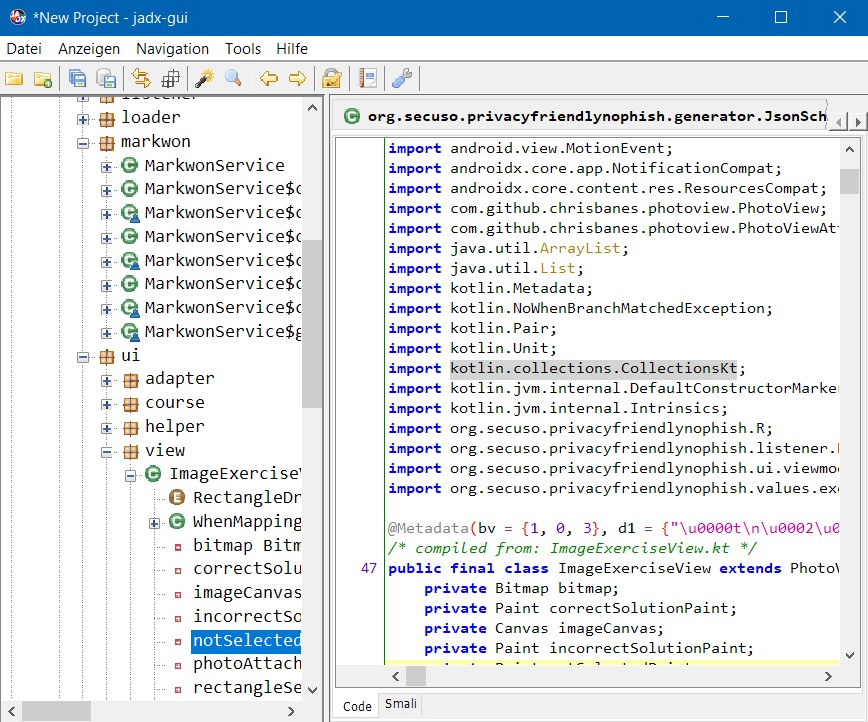
\includegraphics[width=\linewidth]{bilder/jadx.jpg}
    \caption{GUI-Oberfläche von JADX unter Windows 10} % nicht ins Glossar hinzufügen!
    \label{fig:jadx0}
\end{figure}

\section{Neuronale Netze}
In diesem Abschnitt werden die Grundlagen für die Entwicklung von neuronalen Netzen und Autoencodern erläutert.

\subsection{Neuronen und Schichten}
\label{subsec:activation}
Künstliche neuronale Netze sind eine Technologie des maschinellen Lernens. Diese werden laut Goodfellow et al.~\cite[S. 1-2]{goodfellowDeepLearningUmfassende2018} verwendet, um es Computern zu ermöglichen aus Erfahrungen zu lernen. Auf diese Weise können komplexe Konzepte erlernt werden, ohne dass ein Mensch das dafür notwendige Wissen formal beschreiben muss. Neuronale Netze extrahieren dabei Muster aus Rohdaten~\cite[S. 3]{goodfellowDeepLearningUmfassende2018}. An die Funktionsweise des menschlichen Gehirns angelehnt, funktionieren sie, indem künstliche Neuronen miteinander verbunden werden. Diese Neuronen gehen auf die Erfindung des \emph{Perzeptron} durch Rosenblatt~\cite{rosenblattPerceptronProbabilisticModel1958} im Jahr 1958 zurück. Ein solches Perzeptron wird in Abb.~\ref{fig:perceptron} dargestellt.

\begin{figure}[htbp]
    \centering
    \tikzstyle{line} = [draw, -latex']
    \begin{tikzpicture}[
        roundnode/.style={ellipse, draw=black, minimum height=15mm, minimum width=30mm, very thick},
        emptynode/.style={rectangle, very thick, minimum size=5mm},
        ]
        %Nodes
        \node[emptynode] (x1) {$x_1$};
        \node[emptynode] (x0) [above=of x1] {$x_0$};
        \node[emptynode] (x2) [below=of x1] {$x_2$};

        \node[roundnode] (sum) [right=of x1] {$\sum^n_{i=0} w_i * x_i$};
        \node[roundnode] (activation) [right=of sum] {$f(z)$};
        \node[emptynode] (o) [right=of activation] {$o$};
        %Lines
        \path [line] (x0) -- node [midway,above] {$w_0$} (sum);
        \path [line] (x1) -- node [midway,above] {$w_1$} (sum);
        \path [line] (x2) -- node [midway,above] {$w_2$} (sum);

        \path [line] (sum) -- node [midway,above] {$z$} (activation);
        \path [line] (activation) -- node [midway,above] {} (o);
    \end{tikzpicture}
    \caption{Beispielhafte Zusammensetzung eines Neurons mit drei Eingängen und einem Ausgang~\cite[S. 28]{kaulTheoreticalCharacterizationDeep2020}}
    \label{fig:perceptron}
\end{figure}

\pagebreak
Ein Neuron hat beliebig viele Eingänge $n \in \mathbb{N}$, aus welchen eine gewichtete Summe $z$ gebildet wird, die wie folgt definiert ist:

\begin{equation}
    z \coloneq s(x,w) = \sum_{i=0}^n w_i \cdot x_i
\end{equation}


Diese Summe $z$ wird als Eingabe für die sogenannte Aktivierungsfunktion $f(z)$ verwendet. Die Ausgabe der Aktivierungsfunktion ist die des gesamten Neurons. In der Forschungsgemeinschaft wird inzwischen eine Reihe an Aktivierungsfunktionen für die Entwicklung von Autoencodern verwendet. Davon ist die Sigmoid-Funktion eine der am häufigsten genutzten Funktionen. Sie ist eine logistische Funktion, welche sich wegen ihrem charakteristischen Wertebereich [0,1] besonders für neuronale Netze mit Ausgaben aus demselben Wertbereich eignet. Dies ist bei Bildinformationen der Fall, da hier aufgrund der einfacheren Handhabung üblicherweise der ganzzahlige Wertebereich $[0 \isep 255]$ auf das Intervall $[0,1]$ projiziert wird. Die Sigmoid-Funktion ist wie folgt definiert:

\begin{equation}
    \sigma (z) = \frac{1}{1+e^{-z}}
\end{equation}

Eine Funktion mit einem ähnlichen Funktionsgraphen ist der Tangens Hyperbolicus (tanh-Funktion). Dieser hat, anders als die Sigmoid-Funktion, den Wertebereich $[-1,1]$. Nach Goodfellow et al.~\cite[S. 215]{goodfellowDeepLearningUmfassende2018} leistet der Tangens Hyperbolicus normalerweise als Aktivierungsfunktion bessere Arbeit als die Sigmoid-Funktion. Der Tangens Hyperbolicus ist wie folgt definiert:

\begin{equation}
    tanh(z) = \frac{sinh(z)}{cosh(z)} = 1 - \frac{2}{e^{2z}+1}
\end{equation}

Die ReLU-Funktion ist eine sehr häufig genutzte Aktivierungsfunktion. Sie lässt sich sehr leicht optimieren, da ihre Gradienten sowohl groß als auch konsistent sind~\cite[S.~213]{goodfellowDeepLearningUmfassende2018}. Die Funktion entspricht der linearen Einheit im positiven Definitionsbereich und nimmt für $z=0$ und im negativen Definitionsbereich den Wert 0 an.

\begin{equation}
    relu(z) = max\{0, z\}
\end{equation}

\pagebreak
Zur ReLU-Funktion existieren mehrere Generalisierungen, welche ähnlich gut wie oder besser als die ReLU-Funktion funktionieren~\cite[S. 213]{goodfellowDeepLearningUmfassende2018}. In dieser Masterarbeit wird die sogenannte LeakyReLU-Funktion verwendet. Diese unterscheidet sich von der ReLU-Funktion darin, dass sie nicht den Wert 0 im negativen Definitionsbereich annimmt, sondern eine lineare Funktion mit beliebiger Steigung $\alpha$ darstellt. Oft und in dieser Masterarbeit gilt $\alpha = 0,01$. Die LeakyReLU-Funktion ist wie folgt definiert:

\begin{equation}
    leakyrelu(z) =
    \begin{cases}
        z & z > 0 \\
        \alpha z & sonst
    \end{cases}
\end{equation}

In dieser Arbeit werden die ReLU-, LeakyReLU-, Sigmoid- und die tanh-Funktion verwendet. In Abb.~\ref{fig:sigmoid} werden diese Funktionen dargestellt.



\begin{figure}
    \centering
\begin{tikzpicture}[declare function={sigma(\x)=1/(1+exp(-\x));
    sigmap(\x)=sigma(\x)*(1-sigma(\x));}]
    \begin{axis}%
    [
        xmin=-6,
        xmax=6,
        axis x line=bottom,
        ytick={0,.5,1},
        ymax=1,
        axis y line=middle,
        samples=100,
        domain=-6:6,
        legend style={at={(.4,0.9)}}
    ]
        \addplot[blue,mark=none]   (x,{sigma(x)});
        % \addplot[red,dotted,mark=none]   (x,{sigmap(x)});
        \legend{$\sigma(z)$}
    \end{axis}
\end{tikzpicture}
\begin{tikzpicture}[]
    \begin{axis}%
    [
        xmin=-6,
        xmax=6,
        axis x line=bottom,
        ytick={-1,-0.5,0,.5,1},
        ymax=1,
        axis y line=middle,
        samples=100,
        domain=-6:6,
        legend style={at={(.4,0.9)}}
    ]
        \addplot[blue,mark=none]   (x,{tanh(x)});
        % \addplot[red,dotted,mark=none]   (x,{sigmap(x)});
        \legend{$tanh(z)$}
    \end{axis}
\end{tikzpicture}
\begin{tikzpicture}
    \begin{axis}[
        domain=-8:8,
        axis x line=bottom,
        axis y line=middle,
        legend style={at={(.4,0.9)}}
        ]
        \addplot+[mark=none,blue,domain=-8:0] {0};
        \addplot+[mark=none,blue,domain=0:5] {x};
        \legend{$relu(z)$}
    \end{axis}
\end{tikzpicture}
\begin{tikzpicture}
    \begin{axis}[
        domain=-8:8,
        axis x line=middle,
        xtick={-8,-6,-4,-2,0,2,4},
        hide obscured x ticks=false,
        axis y line=middle,
        legend style={at={(.4,0.9)}}
        ]
        \addplot+[mark=none,blue,domain=-8:0] {0.01*x};
        \addplot+[mark=none,blue,domain=0:5] {x};
        \legend{$leakyrelu(z)$}
    \end{axis}
\end{tikzpicture}
\caption{Darstellungen der in dieser Arbeit genutzten Aktivierungsfunktionen (LeakyReLU-Funktion für $\alpha = 0,01$)}
\label{fig:sigmoid}
\end{figure}

In neuronalen Netzen werden Neuronen üblicherweise horizontal und vertikal angeordnet. Auf der horizontalen Ebene werden Netze üblicherweise in Schichten (engl. \emph{Layer}) gegliedert, die auf der vertikalen Ebene miteinander verbunden sind. Diese Schichten bilden zusammen ein neuronales Netz. Insbesondere auf dem Gebiet der Bild- und Sprachverarbeitung hat sich diese Technik durchgesetzt, sodass man oft von tiefen neuronalen Netzen spricht. Dies gilt auch im Kontext dieser Arbeit. Neuronale Netze lassen sich in zwei Gruppen einteilen: Netze, in denen die Verbindungen zwischen Schichten nur in eine Richtung verlaufen (sog. Feedforward-Netze) und \glspl{rnn}, in denen die Verbindungen in Schleifen verlaufen können, um zeitliche Abhängigkeiten abbilden zu können. Am \gls{fzi} werden sogenannte \glspl{ctrnn} erforscht, welche zu den \glspl{rnn} gehören. Mit Hilfe dieser \glspl{ctrnn} soll das automatisierte Testen von \gls{gui}-Oberflächen ermöglicht werden.

\subsection{Lernverfahren}
\label{subsec:lernverfahren}
\todo{Adamax beschreiben}
In dieser Arbeit werden neuronale Netze durch das Verfahren des Gradientenabstiegs mittels Backpropagation nach Rumelhart et al.~\cite{rumelhartLearningRepresentationsBackpropagating1986} trainiert. Dieser Algorithmus funktioniert durch Rückführung des Fehlers der Ausgabe durch das Netz. Daher ist es wichtig zu bestimmen, wie groß der Unterschied zwischen der aktuellen und der gewünschten Ausgabe des Netzes ist. Um dies zu berechnen, werden Fehlerfunktionen verwendet.

\subsubsection{Fehlerfunktionen}
\label{sec:errorfunction}

Die am weitesten verbreitete Fehlerfunktion ist die \glsentrylong{mse}~\cite[S. 15]{yeDeepDiveKeras2022}, die von der tatsächlichen Ausgabe des Netzes $y \in \mathbb{R}^n$ und dem Zielwert $t \in \mathbb{R}^n$ abhängig ist. Die Funktion ist wie folgt definiert:

\begin{equation}
    mse(y,t) = \frac{1}{n} \sum^n_{i=1}(y_i - t_i)^2
\end{equation}

Eine weitere, häufig verwendete Fehlerfunktion ist die \glsentrylong{bce}~\cite{hoRealWorldWeightCrossEntropyLoss2020}. Diese ist ebenfalls von der tatsächlichen Ausgabe des Netzes $y$ und dem Zielwert $t$ abhängig und ist wie folgt definiert:

\begin{equation}
    bce(y,t) = - \frac{1}{n} \sum^n_{i=1}[t_n \cdot \log y_n + (1-t_n) \cdot \log (1-y_n)]
\end{equation}

Die binäre Kreuzentropie ist als Fehlerfunktion beliebter als der \gls{mse}, da die Verwendung des \gls{mse} bei einigen Netzen sehr kleine Gradienten hervorrufen kann~\cite[S. 199]{goodfellowDeepLearningUmfassende2018}. Daher kommt diese Funktion auch zum Training der Netze dieser Arbeit zum Einsatz. Gleichzeitig ist der \gls{mse} als Fehlerfunktion sehr intuitiv und auch ohne tieferes Verständnis der Materie und Entropie durchschaubar. Um die Ausgaben von Netzen zu vergleichen, wird in dieser Arbeit der \gls{mse} verwendet.

\subsubsection{Algorithmus}

Mit dem Verfahren der Backpropagation ist es möglich, neuronale Netze mit mehreren Schichten zu trainieren. Dies funktioniert mittels eines Gradientenabstiegs und wird in Form von Pseudocode unter Algorithmus~\ref{algo:backprop} dargestellt. Hierzu wird eine Eingabe für das Netz vorwärts durch das Netz propagiert und eine Ausgabe berechnet. Diese Ausgabe wird mit der gewünschten Ausgabe verglichen und ein Fehler mittels der oben definierten Fehlerfunktion ermittelt. Das Ziel des Verfahrens ist deren Minimierung. Hierfür wird der ermittelte Fehler entsprechend den Gewichten der einzelnen Neuronen durch das Netz zurückpropagiert. Die Veränderung des Gewichts $\Delta w_{ij}$, wobei $w_{ij}$ das Gewicht des $i$-ten Eingangs des $j$-ten Neurons bezeichnet, berechnet sich wie folgt:

\begin{equation}
    \Delta w_{ij} = - \eta \frac{\partial E}{\partial w_{ij}}
\end{equation}

Hierbei bezeichnet $\eta$ die sogenannte Lernrate. Je größer die Lernrate ist, desto stärker werden die Gewichte $w_{ij}$ angepasst und desto schneller lernt das Netz. Eine zu große Lernrate kann jedoch dazu führen, dass das Netz nicht korrekt lernt. $\Delta w_{ij}$ wird in diesem Fall zu groß und verfehlt das Optimum der Fehlerfunktion, wodurch Instabilitäten entstehen~\cite[S.\,329]{goodfellowDeepLearningUmfassende2018}. Das neue Gewicht $w_{neu}$ berechnet sich dann folgendermaßen:

\begin{equation}
    w_{ij}^{neu} = w_{ij} + \Delta w_{ij}
\end{equation}

\IncMargin{1em}
\begin{algorithm}[htb]


    \KwIn{Eingabewerte $x \in \mathbb{R}^n$ mit Gewichten $w \in \mathbb{R}^{m \times n}$ und Lernrate $\eta \in \mathbb{R}$}
    \KwOut{Angepasster Gewichtsvektor $w_{neu}$}
    \BlankLine
    $z$ $\leftarrow$ 0\\
    \For{$i$ $\leftarrow$ $1$ \KwTo $m$ $\leftarrow$ $\#$ Schichten}{

    \For{$j$ $\leftarrow$ $1$ \KwTo $n$ $\leftarrow$ $\#$ Neuronen in Schicht}{
        \tcc{$f$ ist eine beliebige Aktivierungsfunktion}
        $p \leftarrow \# $ Nachfolger von $j$ in nächster Schicht \\
        $x_j \leftarrow f (\sum^p_{k=1} w_{jk}x_k)$
        % $z$ $\leftarrow$ $z$ + $w_{ij} \cdot x_{ij}$\;
    }
    }
    \BlankLine

    \For{$i$ $\leftarrow$ $1$ \KwTo $n$ $\leftarrow$ $\#$ Neuronen in Schicht}{
        \tcc{Berechne Ergebnis der Fehlerfunktion (Beispiel: \gls{bce})}
        $E(w) \leftarrow bce(x, t)$
    }
    \ForEach{$W$ $\in$ Lagen von Gewichten}{
        \ForEach{$w_{ji} \in W$}{
            $w_{ji} \leftarrow w^{neu}_{ji}$
        }
    }
    \Return{$w_{neu}$}
    \caption{Anpassung der Gewichte mit Backpropagation in einem neuronalen Netz. Hier wird zunächst die Ausgabe einer Schicht bestimmt und dann, mithilfe des Zielvektors, die neuen Gewichte im Netz. \cite[S. 316]{ertelNeuronaleNetze2021}}
    \label{algo:backprop}
\end{algorithm}
\DecMargin{1em}

\pagebreak

\subsubsection{Verwendung von Batches}
Für das Training von neuronalen Netzen werden Eingaben üblicherweise in sogenannte Batches (deutsch Stapel) gruppiert. Diese werden nacheinander durch das Netz propagiert und der Fehler berechnet. Die Gewichte werden erst zum Schluss aktualisiert.

\subsubsection{Optimierungsalgorithmen}
Die Lernrate ist nach Goodfellow et al.~\cite[S.~342]{goodfellowDeepLearningUmfassende2018} ein schwierig einzustellender Parameter. Um diese Auswahl automatisiert treffen zu können, haben sich sogenannte Optimierungsalgorithmen durchgesetzt, die für jeden Parameter eines Netzes eine eigene, dynamische Lernrate berechnen. Wie Goodfellow et al.~\cite[S.~347]{goodfellowDeepLearningUmfassende2018} beschreiben, wird der Optimierungsalgorithmus überwiegend auf Basis persönlicher Präferenzen gewählt. In dieser Arbeit kommt der Algorithmus Adamax zum Einsatz, der bereits in der Bachelorarbeit von Kies~\cite{kiesEntwicklungUndAnalyse2020} zum Einsatz kam. Adamax basiert auf dem Algorithmus Adam von Kingma und Ba~\cite{kingmaAdamMethodStochastic2017}, wobei die $L^\infty$-Norm statt der $L^2$-Norm zum Einsatz kommt.

\section{Convolutional Neural Networks}
\glspl{cnn} sind eine Spezialform der neuronalen Netze, die zur Verarbeitung von Daten mit einer bekannten rasterähnlichen Topologie eingesetzt werden~\cite[S. 369]{goodfellowDeepLearningUmfassende2018}. Bei diesen Netzen kommt die mathematische Operation der Faltung (engl. Convolution) zum Einsatz. Ein neuronales Netz ist ein \gls{cnn}, wenn in mindestens einer Schicht die Faltung als Operation eingesetzt wird~\cite[S. 369]{goodfellowDeepLearningUmfassende2018}.


\subsection{Faltung}
\label{subsec:convolution}


\begin{figure}[p]
    \centering
    \begin{tikzpicture}
        [
        default/.style={rectangle, draw=black, minimum height=7mm,  minimum width=7mm, very thick},
        decodernode/.style={rectangle, draw=green!60, fill=green!10, minimum height=5mm, very thick},
        bottlenecknode/.style={rectangle, draw=blue!60, fill=blue!60, minimum height=5mm, very thick},
        emptynode/.style={rectangle, very thick, minimum size=8mm},
        title/.style={font=\fontsize{6}{6}\color{black!50}\ttfamily},
      ]
      \tikzstyle{l} = [draw, -latex',thick]
        \node (a) [default] { $a$ };
        \node (b) [default, right=0.1cm of a] { $b$ };
        \node (c) [default, right=0.1cm of b] { $c$ };
        \node (d) [default, right=0.1cm of c] { $d$ };
        \node (e) [default, below=0.1cm of a] { $e$ };
        \node (f) [default, right=0.1cm of e] { $f$ };
        \node (g) [default, right=0.1cm of f] { $g$ };
        \node (h) [default, right=0.1cm of g] { $h$ };
        \node (i) [default, below=0.1cm of e] { $i$ };
        \node (j) [default, right=0.1cm of i] { $j$ };
        \node (k) [default, right=0.1cm of j] { $k$ };
        \node (l) [default, right=0.1cm of k] { $l$ };

        \node (w) [default, right=1cm of d] { $w$ };
        \node (x) [default, right=0.1cm of w] { $x$ };
        \node (y) [default, below=0.1cm of w] { $y$ };
        \node (z) [default, right=0.1cm of y] { $z$ };


        % \draw [draw=black!50] (dep.north west) rectangle ($(dep.north east) - (0, 2cm)$);
        \node (input) [draw=black, fit={(a) (b) (e) (f) }, very thick, inner sep=0.5mm] {};
        \node (filter) [draw=black, fit={(w) (x) (y) (z) }, very thick, inner sep=0.5mm] {};

        \node (label1) [emptynode, above=-0.2cm of input.north west, anchor=south west] { Eingabe };
        \node (label2) [emptynode, above=-0.2cm of filter.north west, anchor=south west] { Filter };

        \node (1) [default, align=left, minimum size=2cm, below=1cm of i] { $aw + bx + $\\ $ey + fz$ };
        \node (2) [default, align=left, minimum size=2cm, right=0.2cm of 1] { $bw + cx +$\\ $fy + gz$ };
        \node (3) [default, align=left, minimum size=2cm, right=0.2cm of 2] { $cw + dx +$\\ $gy + hz$ };
        \node (4) [default, align=left, minimum size=2cm, below=0.2cm of 1] { $ew + fx + $\\$iy + jz$ };
        \node (5) [default, align=left, minimum size=2cm, right=0.2cm of 4] { $fw+gx+$\\ $jy+kz$};
        \node (6) [default, align=left, minimum size=2cm, right=0.2cm of 5] { $gw+hx+$\\$ky+lz$ };

        \node (results) [draw=black, fit={(1)}, very thick, inner sep=1mm] {};
        \node (label3) [emptynode, above=-0.2cm of results.north west, anchor=south west] { Ausgabe };

        \draw [l] (input.west) -> ++(-1.5,0) node(upperleft){} |- (results.west);
        \draw [l] (filter.south) -> ++(0,-1.3) node(upperleft){} -- ++(-3.95,0) -- ++(0,-0.35);

      \end{tikzpicture}
    \caption{Beispiel einer Faltung. Dabei werden nur Fälle betrachtet, in denen der Filter vollständig im Bild liegt.~\cite{goodfellowDeepLearningUmfassende2018}}
    \label{fig:conv}
\end{figure}

\begin{figure}[p]
    \centering
    \resizebox*{\textwidth}{!}{\input{convolutional-layer.pdf_tex}}
    \caption{Darstellung der Faltungsoperationen in einer Convolutional-Schicht mit einer Eingabe bestehend aus $k$ Kanälen und $k'$ Filtern}
    \label{fig:conv_layer}
\end{figure}

Bei der Faltung werden im Kontext dieser Masterarbeit ausschließlich zweidimensionale Eingabedaten betrachtet, da es sich hier um Bildinformation handelt. Die Faltungsoperation benötigt zwei Matrizen als Eingabe. Im Fall von \glspl{cnn} ist dies die Eingabe des Netzes $I$ und der sog. Filter $K$ mit Dimension $m \times n$. Abb.~\ref{fig:conv} zeigt das Beispiel einer Faltung, in der die Faltungsoperation auf jeden Eintrag der Eingabe angewendet wird. Die Faltungsoperation ist wie folgt definiert~\cite[S. 371]{goodfellowDeepLearningUmfassende2018}:

\begin{equation}
    S(i,j) = (I * K)(i,j) = \sum_m \sum_n I(m,n) \cdot K(i-m, j-n)
\end{equation}


%Nach Goodfellow et al. wird die Faltung genutzt um und \emph{Parameter Sharing} umzusetzen. Bei Fully-Connected-Schichten wird zwischen den Schichten üblicherweise jedes Neuron einer Schicht mit jedem Neuron der Nachbarschichten verbunden, woraus eine hohe Anzahl an Parametern resultiert. Bei Convolutional-Schichten müssen nur die Parameter des Filters gespeichert werden, wodurch weitaus weniger Gewichte gespeichert werden müssen. Dies wird unter dem Begriff der \emph{spärlichen Interaktionen} zusammengefasst~\cite[S. 374]{goodfellowDeepLearningUmfassende2018}.


\subsection{Convolutional-Schicht}
\label{subsec:conv-layer}
Eine typische Convolutional-Schicht besteht üblicherweise aus drei Phasen. In der ersten Phase werden, wie im vorigen Abschnitt beschrieben, für jeden Eintrag der Eingabe Faltungen durchgeführt. Eine Schicht beinhaltet dabei $k$ Ausgangs-Kanäle, die jeweils einem Filter der Größe $m \times n$ entsprechen. Die Faltungsoperationen einer Schicht werden in Abb.~\ref{fig:conv_layer} dargestellt. Üblicherweise werden in der Literatur noch die Schrittweite $s$ (engl. \emph{Stride}) angegeben. Diese sagt aus, dass ein Filter nicht überall angewendet, sondern nur jede $s$-te Stelle der Ausgabe berechnet wird. Eine solche Schrittweite wird jedoch in dieser Masterarbeit nicht verwendet bzw. auf 1 gesetzt. Dementsprechend existieren pro Schicht $k \times m \times n$ Gewichte, die trainiert werden.
Die Ausgabe nach dieser Phase ist eine Matrix. Deren Dimension werden durch die Höhe $h$ und Breite $w$ der Eingabe, die Anzahl der Filter $k$ und deren Höhe $m$ und Breite $n$ wie folgt bestimmt:




\begin{displaymath}
    h - m + 1 \times w - n + 1 \times k
\end{displaymath}

Die zweite Phase besteht darin, die Ergebnisse der Faltungen als Eingabe für eine nichtlineare Aktivierungsfunktion (siehe Abschnitt~\ref{subsec:activation}) zu verwenden und die Ergebnisse zu berechnen. In der dritten Phase erfolgt üblicherweise ein sogenanntes Pooling. Hierzu existieren verschiedene Ansätze, von denen in dieser Masterarbeit das sog. Max-Pooling umgesetzt wurde. Dabei werden Bildbereiche einer bestimmten Größe (ähnlich dem Filter in Abschnitt~\ref{subsec:convolution}) zusammengefasst und durch den maximalen Wert in diesem Bereich ersetzt. Im Fall der in dieser Masterarbeit untersuchten Netze wird das Max-Pooling verwendet, um die Komplexität der Eingabe zu reduzieren und Information zu komprimieren.


\subsection{Übergang zwischen Schicht-Typen}
\label{subsec:flattening}
Die Ausgabe einer Convolutional-Schicht hat die Dimension $h \times w \times k$. Falls auf diese Schicht jedoch eine Fully-Connected-Schicht folgt, wird eine Eingabe der Dimension $1 \times (h \cdot w \cdot k)$ benötigt. Um dies zu erreichen findet ein sog. \emph{Flattening} statt. Dieses Flattening ignoriert die Dimension der Eingabe und überführt diese in eine Eingabe der gewünschten Dimension.

Falls die alten Dimensionen wiederhergestellt werden müssen, wird das \emph{Reshaping} durchgeführt, das die Eingabe wieder in die alte Dimension $h \times w \times k$ überführt.

\section{Autoencoder}
Autoencoder sind nach Ranzato et al. \cite{ranzatoUnsupervisedLearningInvariant2007} spezielle neuronale Netze, die aus drei Teilen bestehen: Ein Encoder, ein Decoder und ein Bottleneck (auch Repräsentation genannt). Alle Teile werden in Abb.~\ref{fig:autoencoder} dargestellt. Der Encoder sowie der Decoder sind in der Regel neuronale Netze, die von einem schmalen Feature-Vektor separiert werden, dem \emph{Bottleneck}. Das komplette Netz wird so trainiert, dass der Decoder die Eingabe rekonstruiert, \dh, dass die Ausgabe mit der Eingabe übereinstimmt. Da der Decoder nur Zugriff auf das Bottleneck hat und die Eingabe daraus rekonstruieren muss, erlernt der Encoder automatisch die Erstellung einer kodierten Repräsentation der Eingabe im Bottleneck. Da ein Autoencoder nur die Eingabe rekonstruieren muss und keine gelabelten Daten benötigt, zählt das Verfahren zu den unüberwachten Techniken.



Das Ziel der Verwendung eines Autoencoders ist in dieser Masterarbeit das automatische Erlernen einer komprimierten Kodierung von komplexen Daten. Die Qualität der Rekonstruktion ist hierbei abhängig von der Dimension des Bottlenecks. Ist dieses klein gewählt, kann die Eingabe unter Umständen nur unvollständig oder fehlerhaft wiederhergestellt werden.
Falls, wie in der vorliegenden Arbeit, nur eine effiziente Kodierung der Eingabe benötigt wird, kann der Encoder nach dem Training unabhängig vom Decoder verwendet werden.

\begin{figure}[h]
    \centering
    \tikzstyle{line} = [draw, -latex']
    \begin{tikzpicture}[
        encodernode/.style={rectangle, draw=red!60, fill=red!10, minimum height=5mm, very thick},
        decodernode/.style={rectangle, draw=green!60, fill=green!10, minimum height=5mm, very thick},
        bottlenecknode/.style={rectangle, draw=blue!60, fill=blue!60, minimum height=5mm, very thick},
        emptynode/.style={rectangle, very thick, minimum size=5mm},
        ]
        %Nodes
        \node[emptynode] (input) [minimum width=60mm]{Eingabe};
        \node[encodernode] (0) [below=0.2cm of input, minimum width=60mm]{};
        \node[encodernode] (1) [below=0.2cm of 0, minimum width=45mm] {};
        \node[encodernode] (2) [below=0.2cm of 1, minimum width=30mm] {};
        \node[bottlenecknode] (3) [below=0.2cm of 2, minimum width=15mm] {};
        \node[decodernode] (4) [below=0.2cm of 3, minimum width=30mm] {};
        \node[decodernode] (5) [below=0.2cm of 4, minimum width=45mm] {};
        \node[decodernode] (6) [below=0.2cm of 5, minimum width=60mm] {};
        \node[emptynode] (output) [below=0.2cm of 6, minimum width=60mm]{Rekonstruierte Eingabe};

        \node[emptynode] (encoder) [left=1.5cm of 1] {Encoder};
        \node[emptynode] (decoder) [left=1.5cm of 5] {Decoder};
        \node[emptynode] (dummy) [right=2.8cm of 5] {};
        \node[emptynode] (bottleneck) [right=.5cm of 3] {Bottleneck};
    \end{tikzpicture}
    \caption{Darstellung eines Autoencoders~\cite{alvernazAutoencoderaugmentedNeuroevolutionVisual2017}}
    \label{fig:autoencoder}
\end{figure}

Da ein Autoencoder symmetrisch aufgebaut ist, benötigt jede Schicht im Encoder ein Gegenstück im Decoder. Eine Fully-Connected-Schicht im Encoder, die $n$ Neuronen mit $m$ Neuronen verbindet, benötigt daher eine Schicht im Decoder-Teil, die $m$ Neuronen mit $n$ Neuronen verbindet. Ein einfacher, aus Fully-Connected-Schichten bestehender Autoencoder wird in Abb.~\ref{fig:autoencoder_net} dargestellt.


\begin{figure}[h]
    \centering
    \tikzstyle{line} = [draw, -latex']
    \begin{tikzpicture}[
        encodernode/.style={circle, draw=red!60, fill=red!10, minimum height=5mm, very thick},
        decodernode/.style={circle, draw=green!60, fill=green!10, minimum height=5mm, very thick},
        bottlenecknode/.style={circle, draw=blue!60, fill=blue!60, minimum height=5mm, very thick},
        emptynode/.style={rectangle, very thick, minimum size=5mm},
        ]
        %Nodes
        \node[encodernode] (00) {};
        \node[encodernode] [below= 0.3cm of 00] (01) {};
        \node[encodernode] [below= 0.3cm of 01] (02) {};
        \node[encodernode] [below= 0.3cm of 02] (03) {};
        \node[encodernode] [below= 0.3cm of 03] (04) {};
        \node[encodernode] [below= 0.3cm of 04] (05) {};
        \node[encodernode] [below= 0.3cm of 05] (06) {};
        \node[encodernode] [below= 0.3cm of 06] (07) {};
        \node[emptynode] [left= 1.9cm of 00] (x0) {};
        \node[emptynode] [left= 1.9cm of 01] (x1) {};
        \node[emptynode] [left= 1.9cm of 02] (x2) {};
        \node[emptynode] [left= 1.9cm of 03] (x3) {};
        \node[emptynode] [left= 1.9cm of 04] (x4) {};
        \node[emptynode] [left= 1.9cm of 05] (x5) {};
        \node[emptynode] [left= 1.9cm of 06] (x6) {};
        \node[emptynode] [left= 1.9cm of 07] (x7) {};

        \node[encodernode] [right= 1.9cm of 02] (10) {};
        \node[encodernode] [below= 0.3cm of 10] (11) {};
        \node[encodernode] [below= 0.3cm of 11] (12) {};
        \node[encodernode] [below= 0.3cm of 12] (13) {};

        \node[bottlenecknode] [right= 1.9cm of 11] (20) {};
        \node[bottlenecknode] [below= 0.3cm of 20] (21) {};

        \node[decodernode] [right= 1.9cm of 20] (31) {};
        \node[decodernode] [above= 0.3cm of 31] (30) {};
        \node[decodernode] [below= 0.3cm of 31] (32) {};
        \node[decodernode] [below= 0.3cm of 32] (33) {};

        \node[decodernode] [right= 1.9cm of 30] (42) {};
        \node[decodernode] [above= 0.3cm of 42] (41) {};
        \node[decodernode] [above= 0.3cm of 41] (40) {};
        \node[decodernode] [below= 0.3cm of 42] (43) {};
        \node[decodernode] [below= 0.3cm of 43] (44) {};
        \node[decodernode] [below= 0.3cm of 44] (45) {};
        \node[decodernode] [below= 0.3cm of 45] (46) {};
        \node[decodernode] [below= 0.3cm of 46] (47) {};
        \node[emptynode] [right= 1.9cm of 40] (y0) {};
        \node[emptynode] [right= 1.9cm of 41] (y1) {};
        \node[emptynode] [right= 1.9cm of 42] (y2) {};
        \node[emptynode] [right= 1.9cm of 43] (y3) {};
        \node[emptynode] [right= 1.9cm of 44] (y4) {};
        \node[emptynode] [right= 1.9cm of 45] (y5) {};
        \node[emptynode] [right= 1.9cm of 46] (y6) {};
        \node[emptynode] [right= 1.9cm of 47] (y7) {};

        \draw (00) -- (10);
        \draw (00) -- (11);
        \draw (00) -- (12);
        \draw (00) -- (13);
        \draw (01) -- (10);
        \draw (01) -- (11);
        \draw (01) -- (12);
        \draw (01) -- (13);
        \draw (02) -- (10);
        \draw (02) -- (11);
        \draw (02) -- (12);
        \draw (02) -- (13);
        \draw (03) -- (10);
        \draw (03) -- (11);
        \draw (03) -- (12);
        \draw (03) -- (13);
        \draw (04) -- (10);
        \draw (04) -- (11);
        \draw (04) -- (12);
        \draw (04) -- (13);
        \draw (05) -- (10);
        \draw (05) -- (11);
        \draw (05) -- (12);
        \draw (05) -- (13);
        \draw (06) -- (10);
        \draw (06) -- (11);
        \draw (06) -- (12);
        \draw (06) -- (13);
        \draw (07) -- (10);
        \draw (07) -- (11);
        \draw (07) -- (12);
        \draw (07) -- (13);

        \draw (10) -- (20);
        \draw (10) -- (21);
        \draw (11) -- (20);
        \draw (11) -- (21);
        \draw (12) -- (20);
        \draw (12) -- (21);
        \draw (13) -- (20);
        \draw (13) -- (21);

        \draw (20) -- (30);
        \draw (20) -- (31);
        \draw (20) -- (32);
        \draw (20) -- (33);
        \draw (21) -- (30);
        \draw (21) -- (31);
        \draw (21) -- (32);
        \draw (21) -- (33);

        \draw (30) -- (40);
        \draw (30) -- (41);
        \draw (30) -- (42);
        \draw (30) -- (43);
        \draw (30) -- (44);
        \draw (30) -- (45);
        \draw (30) -- (46);
        \draw (30) -- (47);
        \draw (31) -- (40);
        \draw (31) -- (41);
        \draw (31) -- (42);
        \draw (31) -- (43);
        \draw (31) -- (44);
        \draw (31) -- (45);
        \draw (31) -- (46);
        \draw (31) -- (47);
        \draw (32) -- (40);
        \draw (32) -- (41);
        \draw (32) -- (42);
        \draw (32) -- (43);
        \draw (32) -- (44);
        \draw (32) -- (45);
        \draw (32) -- (46);
        \draw (32) -- (47);
        \draw (33) -- (40);
        \draw (33) -- (41);
        \draw (33) -- (42);
        \draw (33) -- (43);
        \draw (33) -- (44);
        \draw (33) -- (45);
        \draw (33) -- (46);
        \draw (33) -- (47);

        \draw [-stealth] (x0) -- (00);
        \draw [-stealth] (x1) -- (01);
        \draw [-stealth] (x2) -- (02);
        \draw [-stealth] (x3) -- (03);
        \draw [-stealth] (x4) -- (04);
        \draw [-stealth] (x5) -- (05);
        \draw [-stealth] (x6) -- (06);
        \draw [-stealth] (x7) -- (07);
        \draw [-stealth] (40) -- (y0);
        \draw [-stealth] (41) -- (y1);
        \draw [-stealth] (42) -- (y2);
        \draw [-stealth] (43) -- (y3);
        \draw [-stealth] (44) -- (y4);
        \draw [-stealth] (45) -- (y5);
        \draw [-stealth] (46) -- (y6);
        \draw [-stealth] (47) -- (y7);
        %Lines
    \end{tikzpicture}
    \caption{Darstellung der Neuronen eines einfachen Autoencoders bestehend aus Fully-Connected-Schichten~\cite{alvernazAutoencoderaugmentedNeuroevolutionVisual2017}}
    \label{fig:autoencoder_net}
\end{figure}

\subsection{Convolutional Autoencoder}
Wenn ein Autoencoder Convolutional-Schichten enthält, spricht man von einem Convolutional Autoencoder, womit der Autoencoder auch zur Gruppe der \gls{cnn} gehört. Die Vorteile beim Einsatz von Convolutional-Schichten wurden in Abschnitt~\ref{subsec:conv-layer} beschrieben.

Ähnlich den Fully-Connected-Schichten, benötigen auch Convolutional-Schichten ein Gegenstück im Decoder, welche das Pooling und die Faltungsvorgänge umkehrt. Daher werden entsprechend Unpooling- und Transposed-Convolution-Phasen (deutsch etwa \emph{Transponierte-Faltungs-Phasen}) benötigt, um das Max-Pooling und die Faltung rückgängig zu machen.

% In dieser Masterarbeit wird nur das Max-Pooling umgesetzt, weshalb an dieser Stelle nur das Max-Unpooling erläutert wird. Das Max-Pooling ist nicht vollständig reversibel, da alle Werte außer dem Maximalwert verloren gehen. Das Max-Unpooling schreibt den Maximalwert an dessen ursprünglichen Index und setzt alle weiteren Werte auf 0. Der ursprüngliche Index des Maximalwertes muss nach dem Max-Pooling entsprechend gespeichert werden.

% Im Anschluss an das Unpooling folgt die transponierte Faltung. Dabei wird gedanklich die Faltung umgekehrt. Der Filter wird auf die Eingabe angewandt, wobei diesmal die Ergebnisse

% \begin{equation}
%     S(i,j) =
% \end{equation}

% \begin{figure}[htbp]
%     \centering
%     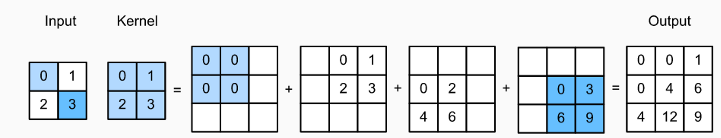
\includegraphics[width=\textwidth]{bilder/transposedconv.png}
%     \caption{Beispiel einer transponierten Faltung}
%     \label{img:transposed_conv}
% \end{figure}

\subsection{Variational Autoencoder}
Der \gls{vae} ist ein Ansatz, der 2014 durch Kingma und Welling~\cite{kingmaAutoEncodingVariationalBayes2014} vorgestellt wurde. Bei diesem Ansatz geht es darum, generative Ansätze mit konventionellen Autoencodern zu verbinden. Ein \gls{vae} unterscheidet sich gegenüber einem konventionellen Autoencoder in zwei Punkten. Zunächst wird am Bottleneck eine zusätzliche Schicht eingefügt, die die Werte im Bottleneck verändert. Darüber hinaus wird die Fehlerfunktion verändert, indem die sogenannte Kullback-Leibler-Divergenz addiert wird.

\subsubsection*{VAE-Schicht}
\label{subsubsec:vae-layer}
Nach dem Encoding-Vorgang wird die letzte Schicht des Encoders in zwei verschiedene Schichten aufgeteilt: die Schicht der Mittelwerte $\mu$ und die der Standardabweichung $\sigma$. Die Schicht der Standardabweichung wird dabei mit einem zufälligen Faktor $\epsilon$ multipliziert und auf die Schicht der Mittelwerte addiert, woraus sich die Werte des Bottlenecks $x$ ergeben. Damit ist $x$ wie folgt definiert:

\begin{equation}
    x = \mu + \epsilon \cdot \sigma
\end{equation}

Die Schichten $\mu$ und $\sigma$ werden im folgenden gemeinsam als \gls{vae}-Schicht bezeichnet und in Abb.~\ref{fig:vae-layer} dargestellt. Durch diesen Vorgang wird ein Rauschen hinzugefügt, durch welches ein Autoencoder die Normalverteilung lernen soll. Aus ähnlichen Werten am Bottleneck sollen ähnliche Ergebnisse resultieren. Das Lernen wird so kontinuierlich~\cite{yeVersatilityAutoencoders2022}.

\begin{figure}[p]
    \centering
    \tikzstyle{line} = [draw, -latex']
    \begin{tikzpicture}[
        encodernode/.style={rectangle, draw=red!60, fill=red!10, minimum height=5mm, very thick},
        decodernode/.style={rectangle, draw=green!60, fill=green!10, minimum height=5mm, very thick},
        bottlenecknode/.style={rectangle, draw=blue!60, minimum height=5mm, very thick},
        emptynode/.style={rectangle, very thick, minimum size=5mm},
        ]
        %Nodes
        \node[emptynode] (input) [minimum width=60mm]{Eingabe};
        \node[encodernode] (0) [below=0.5cm of input, minimum width=70.5mm]{};
        \node[encodernode] (1) [below=0.5cm of 0, minimum width=60.5mm] {};
        \node[encodernode] (2) [below=0.5cm of 1, minimum width=50.5mm] {};
        \node[emptynode] (bottleneck) [below=0.5cm of 2] {};
        \node[emptynode] (bottleneck2) [below=0.1cm of bottleneck] {};

        \node[bottlenecknode] (mu) [right=0.1cm of bottleneck, minimum width=40.5mm] {$\mu$};
        \node[bottlenecknode] (mu2) [below=0.1cm of mu, minimum width=7mm] {$\mu_2$};
        \node[bottlenecknode] (mu1) [left=0.1cm of mu2, minimum width=7mm] {$\mu_1$};
        \node[bottlenecknode] (mu0) [left=0.1cm of mu1, minimum width=7mm] {$\mu_0$};
        \node[bottlenecknode] (mu3) [right=0.1cm of mu2, minimum width=7mm] {$\mu_3$};
        \node[bottlenecknode] (mu4) [right=0.1cm of mu3, minimum width=7mm] {$\mu_4$};

        \node[bottlenecknode] (sigma) [left=0.1cm of bottleneck, minimum width=40.5mm] {$\sigma$};
        \node[bottlenecknode] (sigma2) [below=0.1cm of sigma, minimum width=7mm] {$\sigma_2$};
        \node[bottlenecknode] (sigma1) [left=0.1cm of sigma2, minimum width=7mm] {$\sigma_1$};
        \node[bottlenecknode] (sigma0) [left=0.1cm of sigma1, minimum width=7mm] {$\sigma_0$};
        \node[bottlenecknode] (sigma3) [right=0.1cm of sigma2, minimum width=7mm] {$\sigma_3$};
        \node[bottlenecknode] (sigma4) [right=0.1cm of sigma3, minimum width=7mm] {$\sigma_4$};


        \node[bottlenecknode] (x2) [below=1cm of bottleneck2, minimum width=7mm] {$x_2$};
        \node[bottlenecknode] (x1) [left=0.1cm of x2, minimum width=7mm] {$x_1$};
        \node[bottlenecknode] (x0) [left=0.1cm of x1, minimum width=7mm] {$x_0$};
        \node[bottlenecknode] (x3) [right=0.1cm of x2, minimum width=7mm] {$x_3$};
        \node[bottlenecknode] (x4) [right=0.1cm of x3, minimum width=7mm] {$x_4$};

        \node[bottlenecknode] (real_bottleneck) [below=0.1cm of x2, minimum width=40.5mm] {$x$};
        \node[emptynode] (representation) [left=1.0cm of real_bottleneck, yshift=0.29cm] {Kodierte Repräsentation};

        \node[decodernode] (4) [below=0.5cm of real_bottleneck, minimum width=50.5mm] {};
        \node[decodernode] (5) [below=0.5cm of 4, minimum width=60.5mm] {};
        \node[decodernode] (6) [below=0.5cm of 5, minimum width=70.5mm] {};
        \node[emptynode] (output) [below=0.5cm of 6, minimum width=60mm]{Rekonstruierte Eingabe};

        \draw [-stealth] (sigma0.south) -- (x0.north);
        \draw [-stealth] (sigma1.south) -- (x1.north);
        \draw [-stealth] (sigma2.south) -- (x2.north);
        \draw [-stealth] (sigma3.south) -- (x3.north);
        \draw [-stealth] (sigma4.south) -- (x4.north);
        \draw [-stealth] (mu0.south) -- (x0.north);
        \draw [-stealth] (mu1.south) -- (x1.north);
        \draw [-stealth] (mu2.south) -- (x2.north);
        \draw [-stealth] (mu3.south) -- (x3.north);
        \draw [-stealth] (mu4.south) -- (x4.north);

        \draw [-stealth] (2.south) -- (sigma.north);
        \draw [-stealth] (2.south) -- (mu.north);

        \draw [-stealth] (real_bottleneck.south) -- (4.north);
        \draw [-stealth] (4.south) -- (5.north);
        \draw [-stealth] (5.south) -- (6.north);
        \draw [-stealth] (0.south) -- (1.north);
        \draw [-stealth] (1.south) -- (2.north);


        \node[emptynode] (encoder) [left=2cm of 1, xshift=-0.77cm] {Encoder};
        \node[emptynode] (decoder) [left=2cm of 5, xshift=-0.7cm] {Decoder};
    \end{tikzpicture}
    \caption{Darstellung eines Autoencoders mit der Schicht der Mittelwerte und der Schicht der Standardabweichungen nach Ye~\cite{yeVersatilityAutoencoders2022}}
    \label{fig:vae-layer}
\end{figure}

\subsubsection*{Kullback-Leibler-Divergenz}
\label{subsubsec:kldiv}
Die Kullback-Leibler-Divergenz misst laut Ye~\cite[S. 180]{yeVersatilityAutoencoders2022} das Ausmaß der Divergenz zwischen zwei Verteilungsfunktionen. Bei Betrachtung der Autoencoder würde diese dafür benötigt, eine gleichmäßige und kontinuierliche Verteilung zu lernen und zu verhindern, dass mehrere Cluster entstehen. Die Kullback-Leibler-Divergenz wird dabei auf die Fehlerfunktion addiert und wird minimal, wenn der Mittelwert 0 und die Standardabweichung 1 beträgt. Damit wird das Netzwerk für Clustering und die Reduktion der Standardabweichung bestraft. Die Kullback-Leibler-Divergenz betrachtet zwei Wahrscheinlichkeitsverteilungen $P$ und $Q$ und ist wie folgt definiert~\cite[S. 80]{goodfellowDeepLearningUmfassende2018}:

\begin{equation}
    D_{KL} (P || Q) = \mathbb{E}_{X \sim P} [log \frac{P(x)}{Q(x)}]
\end{equation}

% \begin{itemize}
%     \item Zweck --> Dimensionen reduzieren
%     \item Funktionsweise --> symmetrisches NN
% \end{itemize}
